% !TEX root = ../slides.tex
%%%%%%%%%%%%%%%%%%%%%%%%%%%%%%%%%%%%%%%%%%%%%%%%%%%%%%%%%%%%%%%%%%%%%%%%%%%%%%%%
% Session 8: Introduction: Galerkin vs collocation
%%%%%%%%%%%%%%%%%%%%%%%%%%%%%%%%%%%%%%%%%%%%%%%%%%%%%%%%%%%%%%%%%%%%%%%%%%%%%%%%

\session{session08}{Spectral methods}{Introduction: Galerkin vs collocation}
{Chapter 5}
{\notebook{lectures/spectral/intro}{colocationChebyshev.ipynb}}
{--}

\begin{frame}{Plan for today}
    \begin{enumerate}
        \item Spectral methods vs finite elements.
        \item Two techniques: Galerkin and collocation.
        \item A first example: Chebyshev collocation for Laplace's equation.
        \item Linear algebra of collocation: differentiation matrices.
    \end{enumerate}
    \bigskip
    \takeaway{From now on we follow mostly Canuto, Hussaini, Quarteroni and Zang, \emph{Spectral Methods} (2011).}
\end{frame}

\begin{frame}{Spectral methods vs finite elements}
    Both approximate the solution in a finite-dimensional space $V_N$.
    \medskip
    \begin{center}
        \begin{tabular}{@{}lll@{}}
            \toprule
                         & Finite elements                   & Spectral methods                       \\
            \midrule
            Basis        & local support (pieces)            & global (whole domain)                  \\
            Refinement   & $h \to 0$, fixed degree           & fixed domain, degree $N \to \infty$    \\
            Matrices     & sparse                            & usually full                           \\
            Accuracy     & $O(h^{p})$ for degree $p$         & depends on the smoothness of $u$       \\
            Geometry     & complex domains                   & simple domains (intervals, boxes)      \\
            \bottomrule
        \end{tabular}
    \end{center}
    \medskip
    \textbf{Accuracy of spectral methods} (with periodicity or the right endpoint conditions):
    \begin{itemize}
        \item $u \in C^\infty$: error $O(N^{-m})$ for every $m$ (faster than any power);
        \item $u$ analytic in a neighbourhood of the domain: \alert{geometric} (exponential) convergence, $O(\rho^{-N})$ with $\rho > 1$.
    \end{itemize}
    {\small Spectral-element methods combine both ideas: high degree on each element.}
\end{frame}

\begin{frame}{Galerkin and collocation}
    \begin{enumerate}
        \item \textbf{Galerkin methods.} Keep the variational formulation (as in (E)), but restrict to a finite-dimensional space:
              \[
                  u_N \in V_N, \qquad a(u_N, v_N) = \ell(v_N) \quad \forall v_N \in V_N.
              \]
              Unknowns: the \alert{coefficients} of $u_N$. Requires integrals.
        \item \textbf{Collocation methods.} Choose $V_N$ (e.g.\ polynomials of degree $N$) and \emph{collocation points} $x_j$, and impose the equation \alert{at the points}:
              \[
                  (\text{PDE for } u_N)(x_j) \text{ holds for every } j.
              \]
              Unknowns: the values $u_N(x_j)$ (or the coefficients). No integrals.
    \end{enumerate}
    \begin{remark}[Why ``spectral'']
        The bases are eigenfunctions of differential operators: $e^{ikx}$ for $-\frac{\diff^2}{\diff x^2}$; orthogonal polynomials for singular \emph{Sturm--Liouville} operators. We use them for general operators.
    \end{remark}
\end{frame}

\begin{frame}{Collocation for Laplace's equation}
    \[
        -u''(x) = f(x) \quad \text{in } (-1,1), \qquad u(-1) = u(1) = 0.
    \]
    \begin{itemize}
        \item Look for $u_N \in \R_N[x]$: $N+1$ unknown coefficients.
        \item Choose $N+1$ points $1 = x_0 > x_1 > \cdots > x_N = -1$ and impose
              \[
                  \begin{cases}
                      -u_N''(x_j) = f(x_j), & j = 1, \dots, N-1, \\
                      u_N(-1) = u_N(1) = 0.
                  \end{cases}
              \]
        \item We can use any basis, e.g.\ monomials $u_N = \sum_{k=0}^N c_k x^k$.
    \end{itemize}
    \bigskip
    \textbf{Question.} Which points? Which basis?
    \takeaway{Equi-distant points are a bad idea (Runge's phenomenon, Session 10).}
\end{frame}

\begin{frame}{Chebyshev--Gauss--Lobatto points}
    \begin{columns}[c]
        \begin{column}{.55\textwidth}
            \[
                x_j = \cos\frac{j\pi}{N}, \qquad j = 0, \dots, N .
            \]
            \begin{itemize}
                \item Projections of equi-spaced points on the half circle.
                \item They cluster near $\pm 1$.
                \item Natural basis: Chebyshev polynomials
                      \[
                          T_k(x) = \cos(k \arccos x),
                      \]
                      and we write $u_N = \sum_{k=0}^N a_k T_k$.
                \item $T_k(x_j) = \cos\frac{kj\pi}{N}$: the system is easy to write.
            \end{itemize}
        \end{column}
        \begin{column}{.42\textwidth}
            \centering
            \begin{tikzpicture}[scale=2]
                \draw[gray] (1,0) arc (0:180:1);
                \draw[-{Stealth}] (-1.15,0) -- (1.2,0);
                \foreach \j in {0,...,10} {
                    \pgfmathsetmacro{\ang}{180*\j/10}
                    \draw[dotted,blue] ({cos(\ang)},{sin(\ang)}) -- ({cos(\ang)},0);
                    \fill[blue] ({cos(\ang)},{sin(\ang)}) circle (.6pt);
                    \fill[red] ({cos(\ang)},0) circle (.9pt);
                }
                \node[below] at (-1,0) {\scriptsize $-1$};
                \node[below] at (1,0) {\scriptsize $1$};
                \node at (0,-.3) {\scriptsize $N = 10$};
            \end{tikzpicture}
        \end{column}
    \end{columns}
\end{frame}

\begin{frame}{Very fast convergence}
    \begin{columns}[c]
        \begin{column}{.58\textwidth}
            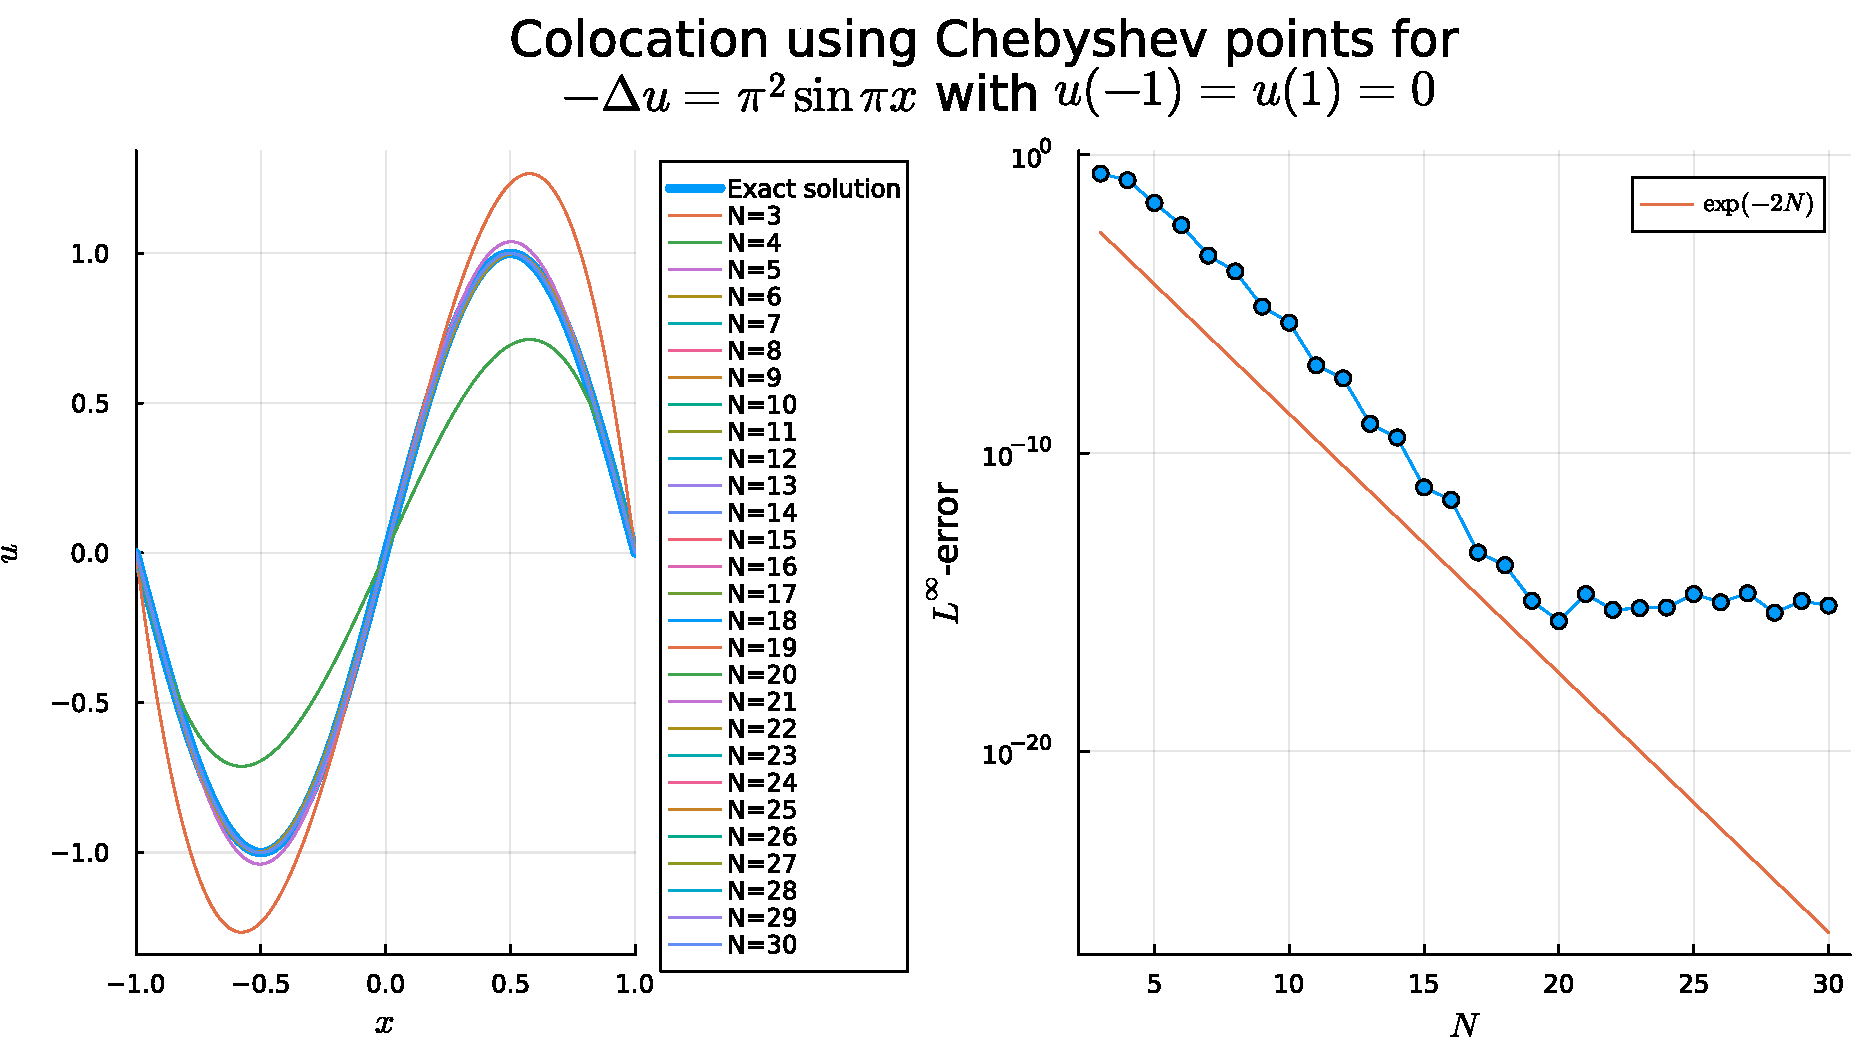
\includegraphics[width=\textwidth]{../../lectures/spectral/intro/convergenceChebyshev.pdf}
        \end{column}
        \begin{column}{.4\textwidth}
            \begin{itemize}
                \item Maximum error of Chebyshev collocation (sampled on a fine uniform grid) for a smooth (sine) solution.
                \item The error decays faster than any power of $N$, until it reaches \alert{machine precision}.
                \item Compare: linear finite elements give $O(h^2) = O(N^{-2})$.
            \end{itemize}
        \end{column}
    \end{columns}
\end{frame}

\begin{frame}{Linear algebra: coefficients and values}
    Basis $\phi_{k}$, $k \in Z_N = \{k_0, \dots, k_N\}$, and $u_N(x) = \sum_{k \in Z_N} \hat u_k \phi_k(x)$.
    \begin{itemize}
        \item Galerkin methods give equations for the \alert{coefficients} $\hat u_k$.
        \item Collocation methods give equations for the \alert{values} $u_N(x_j)$.
    \end{itemize}
    They are related by the matrix $\mat A_N = \big(\phi_{k}(x_j)\big)_{j,k}$:
    \[
        \begin{pmatrix} u_N(x_0) \\ \vdots \\ u_N(x_N) \end{pmatrix}
        =
        \underbrace{\begin{pmatrix}
            \phi_{k_0}(x_0) & \cdots & \phi_{k_N}(x_0) \\
            \vdots          &        & \vdots          \\
            \phi_{k_0}(x_N) & \cdots & \phi_{k_N}(x_N)
        \end{pmatrix}}_{\mat A_N}
        \begin{pmatrix} \hat u_{k_0} \\ \vdots \\ \hat u_{k_N} \end{pmatrix}.
    \]
    \begin{itemize}
        \item Values are good for plotting; to recover the coefficients use $\mat A_N^{-1}$.
    \end{itemize}
\end{frame}

\begin{frame}{Differentiation matrices}
    In our spectral bases, the derivative of a basis function is in $V_N$:
    \[
        \begin{pmatrix} \phi_{k_0}'(x) \\ \vdots \\ \phi_{k_N}'(x) \end{pmatrix}
        = \mat B_N^t
        \begin{pmatrix} \phi_{k_0}(x) \\ \vdots \\ \phi_{k_N}(x) \end{pmatrix}
        \quad \Longrightarrow \quad
        u_N'(x) = (\phi_{k_0}(x), \dots, \phi_{k_N}(x))\, \mat B_N \vec{\hat u}_N .
    \]
    Evaluating at the nodes:
    \[
        \begin{pmatrix} u_N'(x_0) \\ \vdots \\ u_N'(x_N) \end{pmatrix}
        = \underbrace{\mat A_N \mat B_N \mat A_N^{-1}}_{\mat D_N}
        \begin{pmatrix} u_N(x_0) \\ \vdots \\ u_N(x_N) \end{pmatrix},
        \qquad
        \begin{pmatrix} u_N''(x_0) \\ \vdots \\ u_N''(x_N) \end{pmatrix}
        = \mat D_N^2
        \begin{pmatrix} u_N(x_0) \\ \vdots \\ u_N(x_N) \end{pmatrix}.
    \]
    \begin{itemize}
        \item If the basis is orthogonal, $\mat B_N$ is easy to compute.
        \item For Chebyshev--Gauss--Lobatto points, $\mat D_N$ is known explicitly (Canuto et al., Section 2.4).
    \end{itemize}
\end{frame}

\begin{frame}{The collocation system in matrix form}
    Find $u_N \in \R_N[x]$ such that $-u_N''(x_j) = f(x_j)$ for $j = 1, \dots, N-1$, and $u_N(x_0) = g(x_0)$, $u_N(x_N) = g(x_N)$.
    \[
        \begin{pmatrix}
            \vec e_0^{\,t}             \\
            -\mat Z_N \mat D_N^2 \\
            \vec e_N^{\,t}
        \end{pmatrix}
        \begin{pmatrix}
            u_N(x_0) \\ u_N(x_1) \\ \vdots \\ u_N(x_{N-1}) \\ u_N(x_N)
        \end{pmatrix}
        =
        \begin{pmatrix}
            g(x_0) \\ f(x_1) \\ \vdots \\ f(x_{N-1}) \\ g(x_N)
        \end{pmatrix},
    \]
    \begin{itemize}
        \item $\vec e_0, \vec e_N$: first and last vectors of the canonical basis of $\R^{N+1}$;
        \item $\mat Z_N = (\vec 0 \mid \mat I_{N-1} \mid \vec 0) \in \R^{(N-1)\times(N+1)}$ extracts the interior rows.
    \end{itemize}
    \takeaway{Boundary conditions replace the equations at the boundary nodes.}
\end{frame}

\begin{frame}{Galerkin vs collocation}
    \begin{center}
        \begin{tabular}{@{}lll@{}}
            \toprule
                                   & Galerkin                         & Collocation                       \\
            \midrule
            Equation imposed       & tested against $V_N$             & at the collocation points         \\
            Natural unknowns       & coefficients $\hat u_k$          & point values $u_N(x_j)$           \\
            Needs                  & integrals (quadrature)           & point evaluations                 \\
            Analysis               & Céa, Aubin--Nitsche              & quadrature rules (Sessions 10--11)\\
            Non-linear terms       & convolutions of coefficients     & point-wise products               \\
            \bottomrule
        \end{tabular}
    \end{center}
    \bigskip
    \textbf{Time-dependent problems.} For the heat equation $u_t = u_{xx}$ the same reasoning gives a semi-discretisation in space:
    \[
        \frac{\diff}{\diff t} u_N(t, x_j) = \big(\mat D_N^2\, \vec u(t)\big)_j, \qquad j = 1, \dots, N-1,
    \]
    plus boundary conditions at $x_0$, $x_N$: a system of ODEs.
\end{frame}

\begin{frame}{Summary and practice}
    \begin{itemize}
        \item Spectral methods: global bases, very fast convergence for smooth solutions.
        \item Galerkin: variational formulation on $V_N$. Collocation: equation at the nodes.
        \item Collocation in practice: values at the nodes, differentiation matrix $\mat D_N = \mat A_N \mat B_N \mat A_N^{-1}$.
        \item Chebyshev--Gauss--Lobatto points $x_j = \cos(j\pi/N)$ avoid the problems of equi-distant points.
    \end{itemize}
    \bigskip
    \textbf{Practice.}
    \begin{itemize}
        \item Notebook \notebook{lectures/spectral/intro}{colocationChebyshev.ipynb}: solve $-u'' = f$ by Chebyshev collocation and plot the error as a function of $N$.
    \end{itemize}
    \bigskip
    \textbf{Next session:} Fourier series.
\end{frame}
